\documentclass[../main/report.tex]{subfiles}
\begin{document}

\chapter{GPU}

The GPU is at the heart of the Demolicious system.
Inspired by SIMD and SIMT architecture and programming models, the GPU architecture is named 'GhettoCUDA' in honor of NVIDIAs CUDA environment.\todo{cite this}

The GhettoCUDA architecture is highly parallel, in that it allows for a great number of threads to execute in parallel on multiple streaming processors.
A thread is the unit of execution, in essence a single procedure, that when correctly parameterized by run-time values allows for the transformation of a set of input data to a graphical representation to be visualized by the HDMI module.
A simple kernel, requiring no input, might be one that for each pixel in the framebuffer stores the color red.

The main design challenge in creating a GPU-inspired system is managing to saturate the memory bus as much as possible, changing memory access patterns from clustering together in time to a more spread-out pattern.
To facilitate this, the architecture allowing for multiple threads to execute on each streaming processor core, with a staggered start.
This design decision allows for a steady stream of load/store instructions without requiring a system stall as one waits for memory requests to return.

\section{Responsibilities}

The GPU has a relatively simple job:
\begin{enumerate}
  \item
    Receive instructions and constant data from the MCU
  \item
    Receive kernel invocations from the MCU
  \item
    Write results to external SRAM
  \item
    Assert the 'computation finished' signal to the MCU
\end{enumerate}

\section{Architecture Overview}
\begin{figure}[H]
\centering
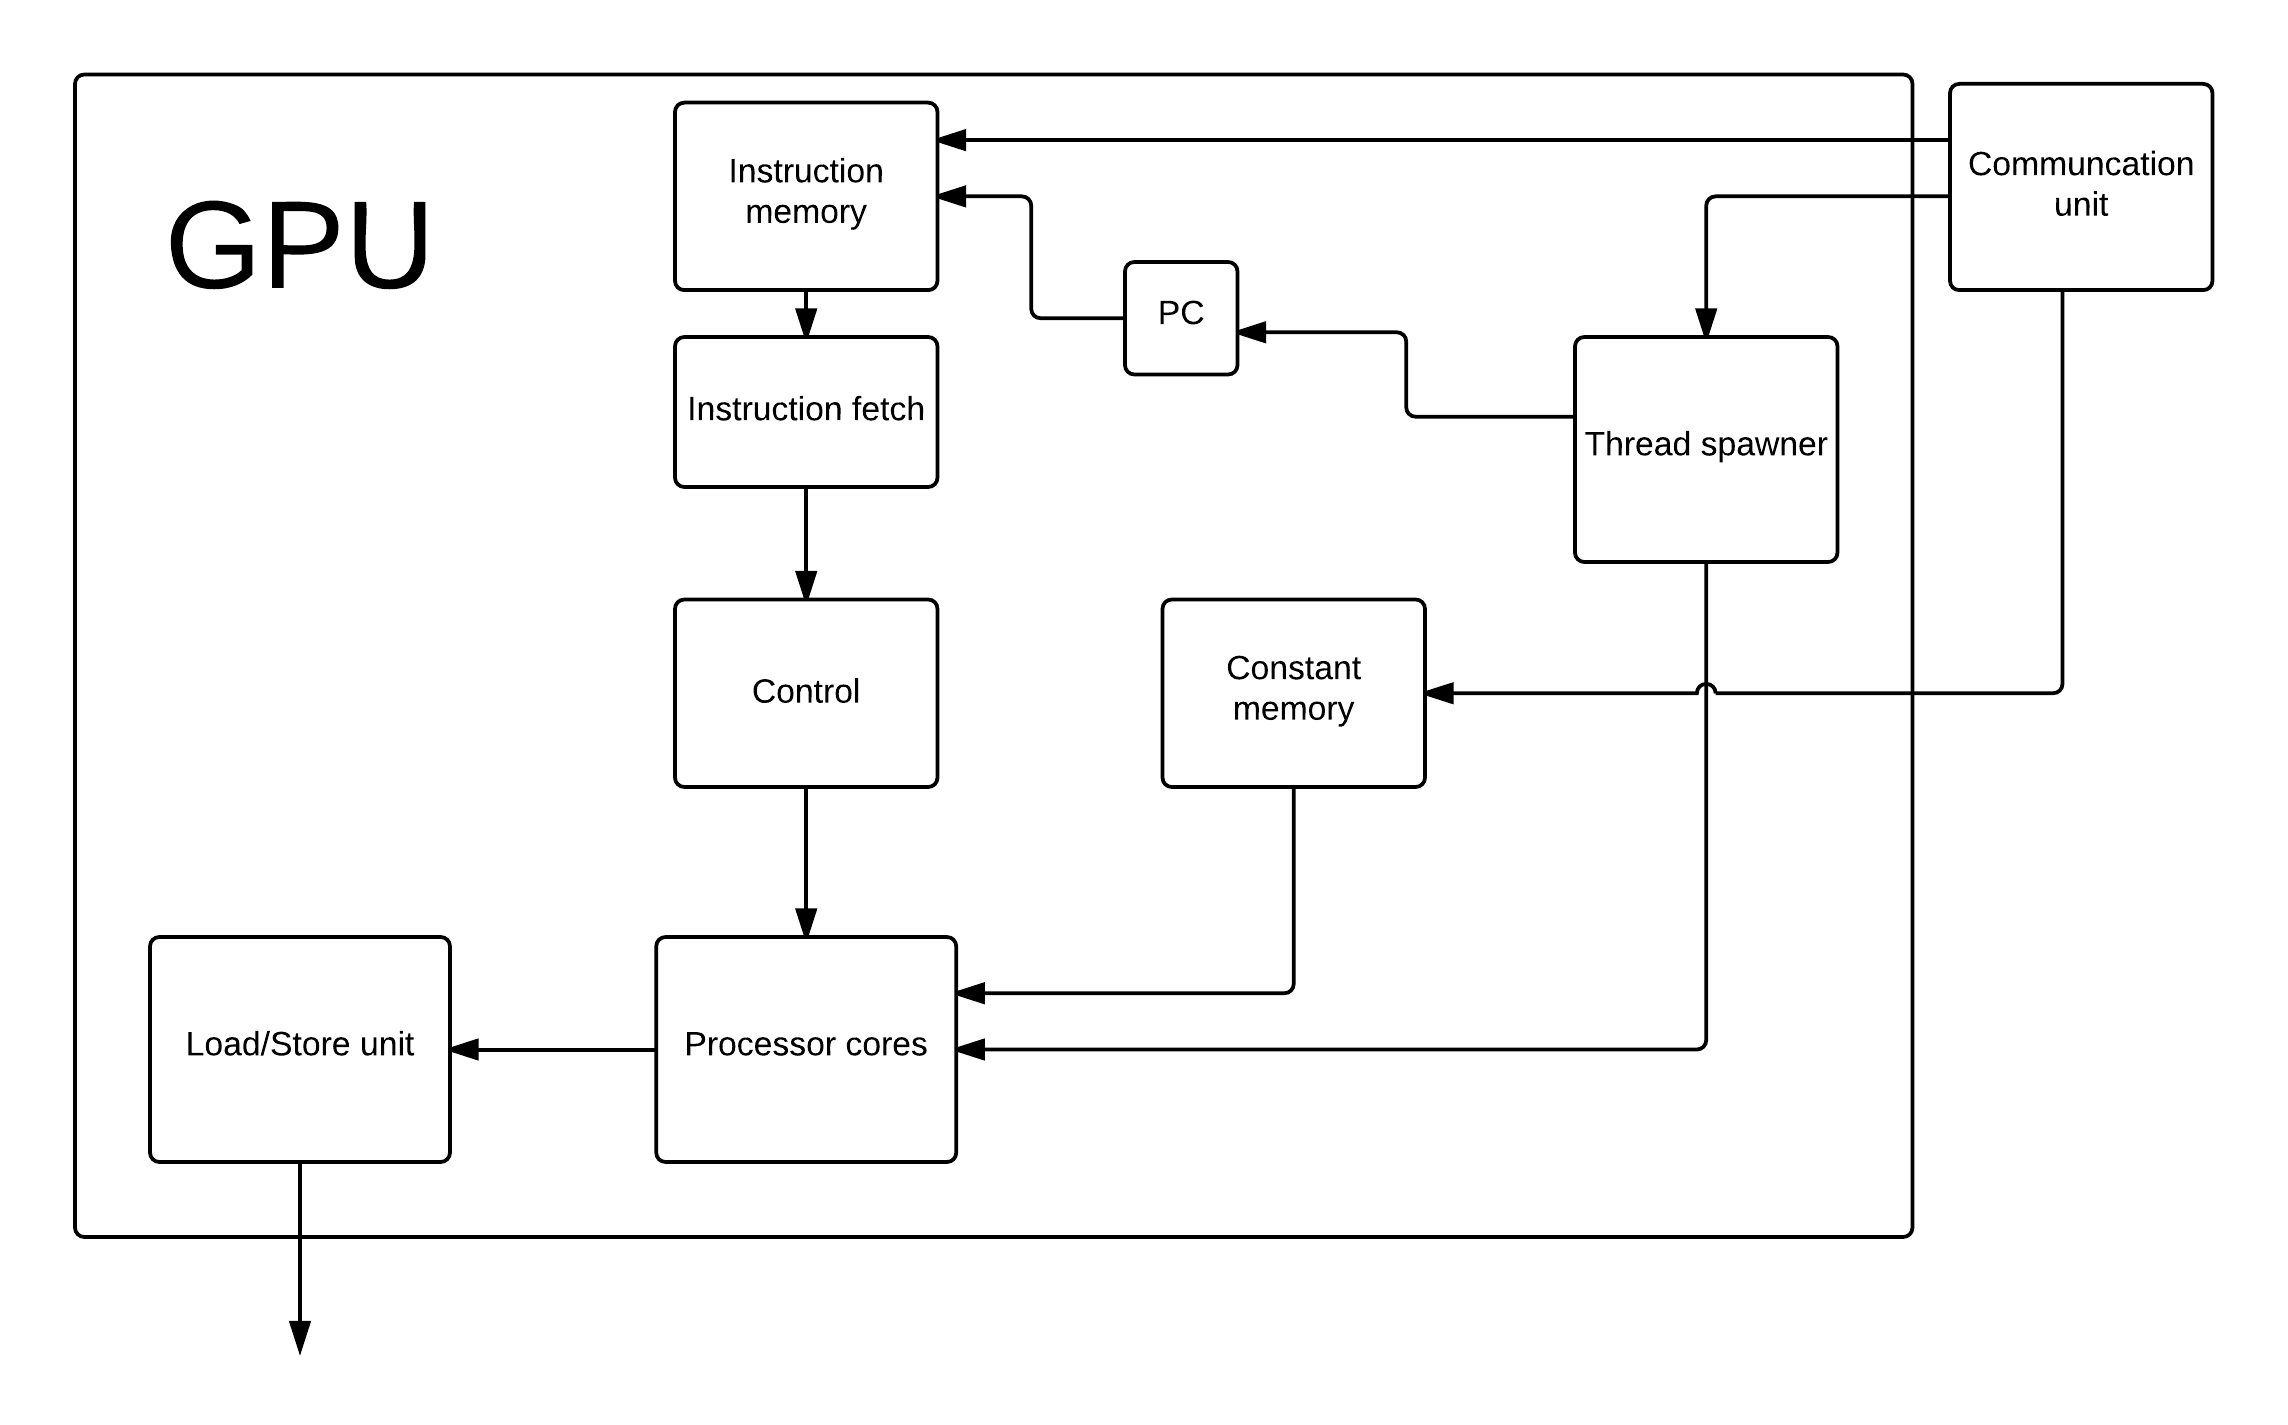
\includegraphics[width=\textwidth]{../gpu/diagrams/architecture_overview.png}
\caption{A high level overview of the GPU.}
\label{fig:architecture_overview}
\end{figure}
Figure \ref{fig:architecture_overview} presents a high level overview over the data-flow in the GPU.
The CPU issues commands to the GPU via the communication unit. Commands include actions such as launching a kernel, uploading kernels to the instruction memory, and writing to the constant memory.
Instructions are fetched from the instruction memory and decoded by the control unit, which has the responsibility of setting the control signals for the instructions.
The processors load constants from the constant memory, and uses the load/store unit for  accessing the data memory. 


\section{Kernel Structure}

\section{Receiving a Kernel Call}
\begin{figure}[H]
\centering
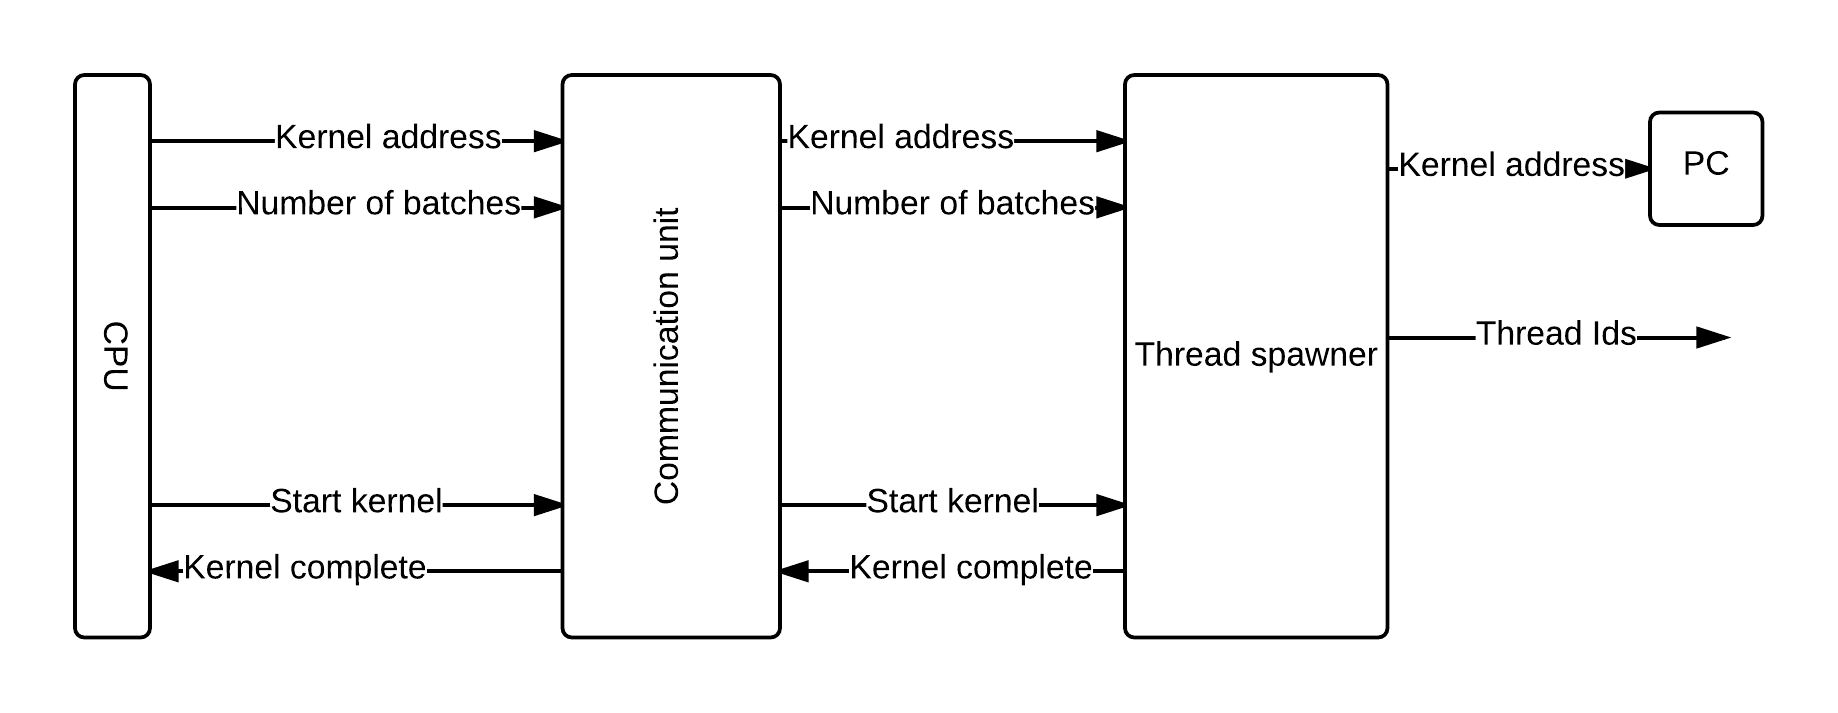
\includegraphics[width=\textwidth]{../gpu/diagrams/receiving_a_kernel_call.png}
\caption{Launching a kernel from the GPU's viewpoint.}
\label{fig:kernel_call}
\end{figure}

The communication unit is responsible for receiving kernel call requests from the CPU, and initiating the request.
A valid kernel call consists of the address of the kernel, the number of batches to launch, and asserting the launch signal.

The kernel launch signals are forwarded to the thread spawner, which writes the kernel start address to the PC register, and starts distributing threadIDs to the streaming processors. 
After holding the kernel launch signals high for one clock cycle, the communication unit has completed its role in launching the kernel.
When the kernel completes executing, the thread spawner asserts the kernel done signal, and the communication unit forwards the signal to the CPU, indicating that the kernel call has completed.


\section{Running a Kernel}
Once the thread spawner has been initiated by the communication unit, the kernel runs to completion without intervention by the CPU. 
At the beginning of a kernel run, the thread spawner assigns threadIDs to each warp in the barrel.
After the initial IDs have been assigned the GPU enters normal execution.
\begin{figure}[H]
	\centering
	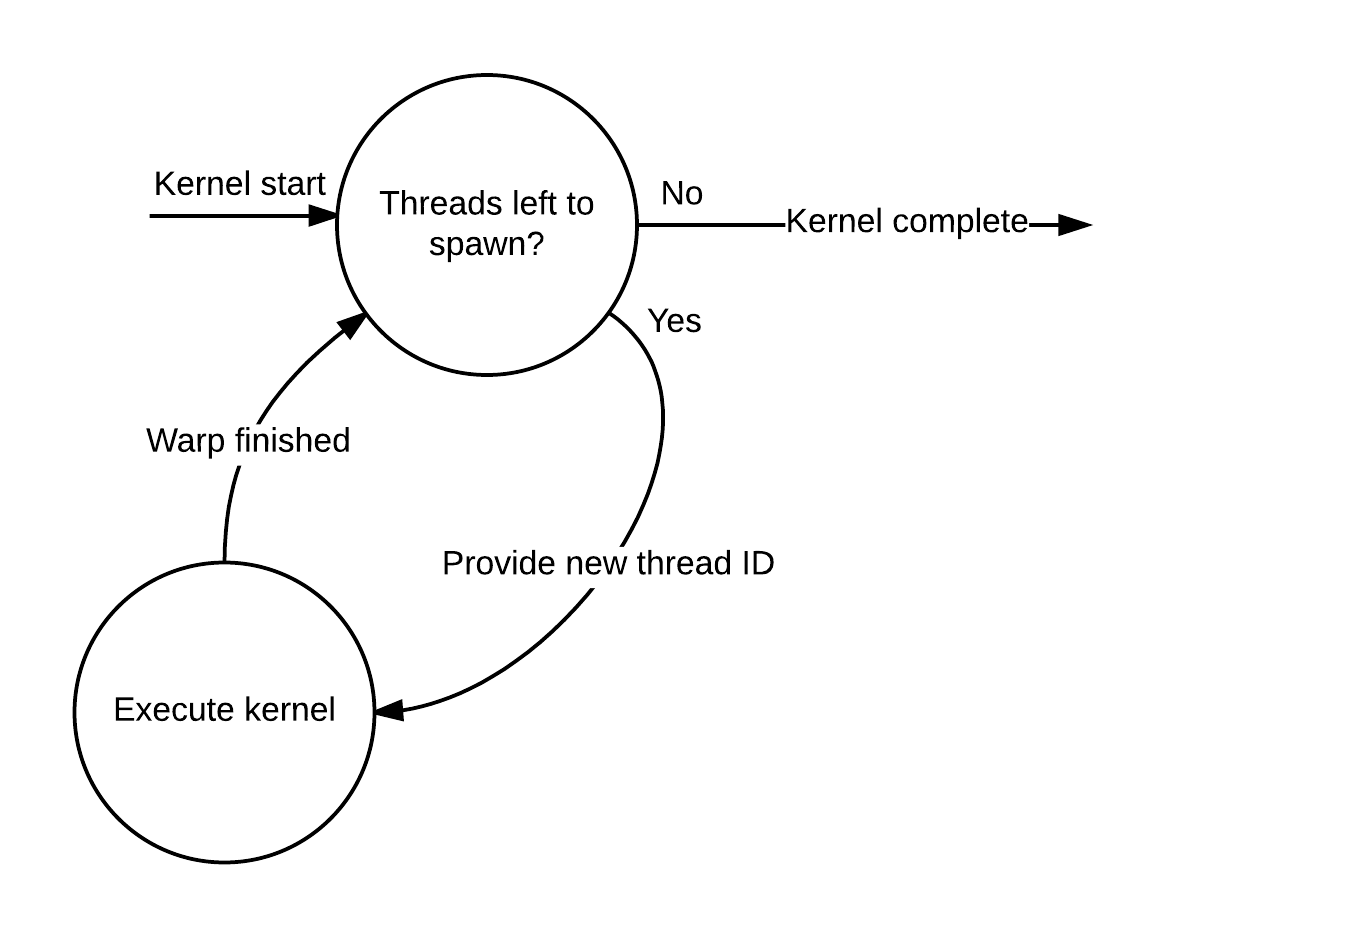
\includegraphics[width=0.9\textwidth]{../gpu/diagrams/kernel_run_state_machine.png}
	\caption{The GPU's internal state during kernel execution.}
	\label{fig:kernel_run_state_machine}
\end{figure}
A normal kernel execution can be represented by the state machine in figure \ref{fig:kernel_run_state_machine}.
During the kernel execution stage the warps execute the same instructions in lock-step one warp at a time, until the control unit encounters a \textit{Finished} instruction.
Upon receiving a \textit{Finished} instruction the control unit asserts the finished signal alerting the thread spawner that the warp requires new threadIDs.
The thread spawner keeps track of the number of threads awaiting launch.
When the thread spawner receives a \textit{Finished} instruction and no more threads are awaiting launch, the kernel run has completed.

\section{Component Details}

\todo{Can this be called something else? It's kind of confused with the component details in the PCB chapter}

\subsection{Processor Core}

\begin{figure}[H]
	\centering
	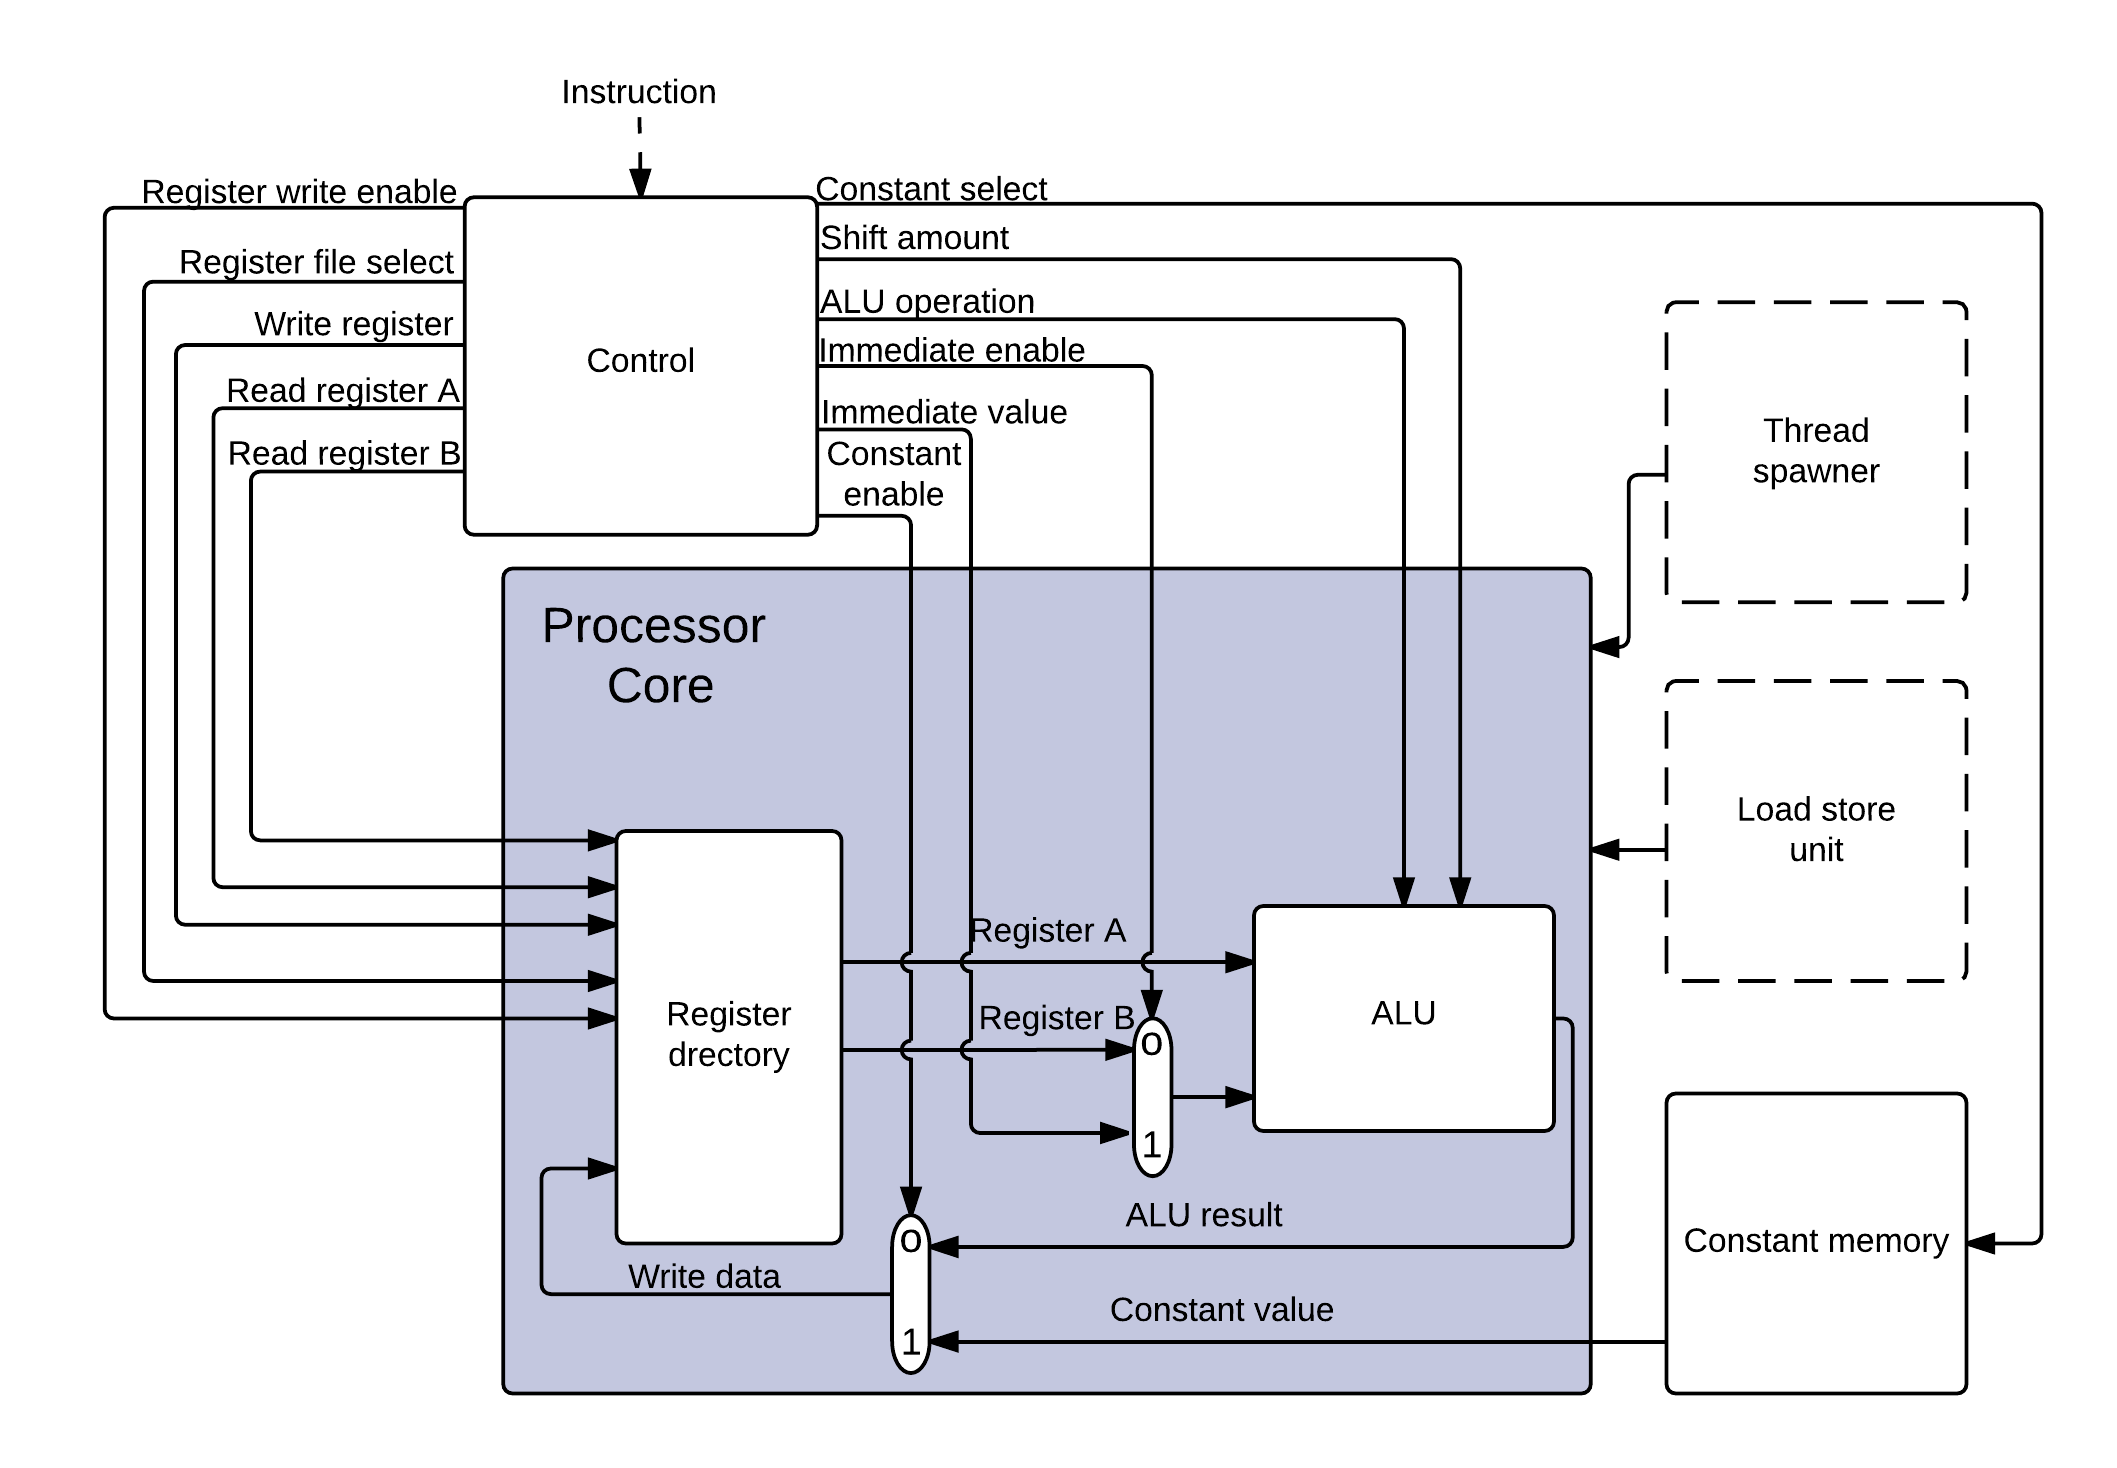
\includegraphics[width=1.2\textwidth]{../gpu/diagrams/processor_core.png}
	\caption{A single processor core.}
	\label{fig:processor_core}
\end{figure}

Each processor core contains an ALU and a register directory.
On each clock cycle the ALU receives the selected values from the register directory.
On the same cycle, the value is written back to the register selected by the control unit.

If the current instruction is a load constant instruction, the control unit selects which constant to fetch from constant memory.
The constant enable signal is asserted, causing the multiplexer to select the constant value as the write back value.
The constant memory is stored on chip, meaning it returns the constant on the same cycle as it is requested.

To perform immediate instructions, the control unit asserts the immediate enable signal.
The immediate value is then selected by the multiplexer and used as an operand in the ALU.



\subsection{Thread Spawner}

The thread spawner is responsible for converting the MCUs request of n kernels executing kernel k on data set d to actual hardware threads.
As all kernels are uniquely identifiable by their respective thread ID, the thread spawner is responsible for providing strictly increasing and unique IDs.


\subsection{Register Directory}

\subsection{Load/Store Unit}

\end{document}
